\documentclass[a4paper,12pt]{article}
\usepackage{graphicx}
\usepackage[dvipsnames]{xcolor}
\usepackage{wrapfig}
\usepackage{color}
\usepackage{graphicx}
\usepackage{subfigure}
\usepackage{multirow}
\usepackage[section] {placeins}
\usepackage{tikz}
\usepackage{amsmath}
\usetikzlibrary{matrix,calc}
\usetikzlibrary{positioning}
\usetikzlibrary{matrix}
\pgfdeclarelayer{background}
\pgfsetlayers{background,main}
\usepackage[hidelinks]{hyperref}

\definecolor{darkred}{rgb}{0,0,0.5}
\definecolor{darkgreen}{rgb}{0,0.5,0}
\definecolor{darkblue}{rgb}{0.5,0,0}
\hypersetup{ colorlinks, linkcolor=darkblue, filecolor=darkgreen, urlcolor=darkred, citecolor=darkblue}

\begin{document}
\begin{titlepage}
\begin{center}
	\textsc{\LARGE Indian Institute of Technology
			\\Bombay} \\[2.5cm]
	\begin{figure}[ht!]
	\begin{center}
		
\includegraphics[scale = 1.4]{images/1}
	\end{center}
	\end{figure}

    \vspace*{-0.6cm}
	\hrule \hrule \hrule
	\vspace{0.5cm}	
	\textsc{\Large CS 492 : BTP Stage I}\\[0.5cm]
	% Title
	{\huge \bfseries Erlang Distributed File System (eDFS)} \\[0.5cm]
	\hrule \hrule \hrule
	\vspace{4cm}
	
	% Author and supervisor
	\begin{minipage}{0.4\textwidth}
	\begin{flushleft} \large
		\emph{By:} \\
		Aman Mangal (100050015)
	\end{flushleft}
	\end{minipage}
	\begin{minipage}{0.4\textwidth}
	\begin{flushright} \large
		\emph{Coordinator:} \\
		Prof. G. Sivakumar
	\end{flushright}
	\end{minipage}
	\vspace{0.5cm}
	
	% Bottom of the page
	{\large \today}
\end{center}
\end{titlepage}
\tableofcontents
\vspace{0.5cm}
\hrule \hrule \hrule
\newpage

\section{Introduction}
Distributed File System is an extension of File System which manages files and data on multiple storage devices and provides more performance and reliability using various modern techniques. Outside world only sees it as a single storage device and thus simplifying the interface to a great extent. It also provides location transparency and redundancy to improve data availability in case of failure or heavy load.

The idea of eDFS is to use Erlang distributive capabilities and build a fault tolerant, highly scalable and reliable distributed file system. We keep in mind the following assumptions while designing eDFS just like Google File System (GFS) \cite{ghemawat03} -
\begin{enumerate}
\item Component failures are norm rather than exception.
\item Files are huge by traditional standards.
\item Most files are mutated by appending rather than overwriting existing data, we may support concurrent append in future
\item Sequential access are more compared to random access. We optimize the file system for stream access.
\end{enumerate}

We prefer performance over security as of now. We support the usual operations to create, delete, open, close, read and write files.

\section{Design Overview}
\subsection{Architecture}
A cluster of eDFS contains a master node, many worker nodes and one or more than one client servers as shown in figure \ref{edfs_design} on page \pageref{edfs_design}. Client communicate with client server in order to perform operations on file system. Client can be a browser or any other application which can communicate over tcp/ip connection. Client server can directly communicate to master node or any worker node. Multiple clients can perform operations on file system at the same time. Multiple client servers can be deployed for load balancing.
\begin{figure}[h]
  \begin{center}
    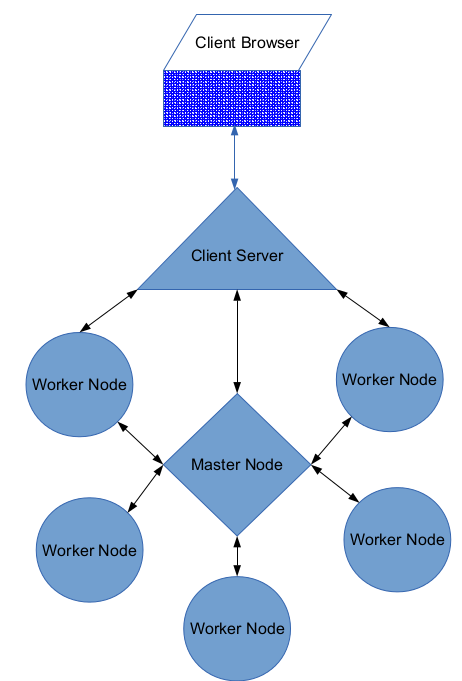
\includegraphics[scale = 0.5]{images/design}
  \end{center}
  \caption{eDFS design}
  \label{edfs_design}
\end{figure}

\subsection{Master node (Metadata Server)}
Master node takes care of handling metadata. It is stored in mnesia in ets tables only. Each file is divided into chunks of equal size. Every chunk is assigned a unique id and stored on multiple worker node based on the replication factor of the file. Following is the table sotred in mnesia-
\begin{table}[h]
\centering
\begin{tabular}{|c|}
\hline 
name \\ 
\hline 
replication factor \\ 
\hline 
chunks \\ 
\hline 
\end{tabular} 
\end{table}

\begin{itemize}
\item \textbf{Name:} name of the file
\item \textbf{Replication Factor:} number of replicas of each chunk
\item \textbf{Chunks:} list of all the chunks of the file stored as \{id, byte begin, byte end, replicas\}
\item \textbf{Id:} chunk id
\item \textbf{Byte begin:} byte number of first byte in the chunk
\item \textbf{Byte end:} byte number of last byte in the chunk
\item \textbf{Replicas:} list of worker ids where replication of the chunk are stored
\end{itemize}

We may support multiple master node and replication of metadata in future.

\subsection{Generation of Chunk Id}
Chunk id is a unique randomly generated string. The chunk is stored with the same name on every worker node. The name can only contain letters a-z, A-Z, 0-9, ".", "\_" (64 letters). It is assumed that name is calculated with less than a million per sec frequency.  Timestamp from operating system is converted into an equivalent representation of a random string and used as the name of a chunk. It is represented using 8 letters (~64 bits). It is possible to generate such ids upto year of 2170 which is approximately 200 years later than the time since when cpu counts the number of seconds (1970).

\subsection{Worker Node}

\section{System Interaction}
\subsection{OTP Hierarchy}
\subsection{Data Flow}
\subsection{Data Replication}
\subsection{Garbage Collection}

\section{Additional Features}

\section{Graphical User Interface}

\section{Testing}
\subsection{Map Reduce}

\begin{thebibliography}{9}
\bibitem{ghemawat03}
  \textsc{Sanjay Ghemawat, Howard Gobioff and Shun-Tak Leung}.
  The Google file system.
  \emph{In SOSP '03: Proceedings of the nineteenth ACM symposium on Operating systems principles}
  New York, NY, USA, 2003
\end{thebibliography}

\end{document}
